% Options for packages loaded elsewhere
\PassOptionsToPackage{unicode}{hyperref}
\PassOptionsToPackage{hyphens}{url}
%
\documentclass[
  english,
  man,floatsintext]{apa6}
\usepackage{lmodern}
\usepackage{amsmath}
\usepackage{ifxetex,ifluatex}
\ifnum 0\ifxetex 1\fi\ifluatex 1\fi=0 % if pdftex
  \usepackage[T1]{fontenc}
  \usepackage[utf8]{inputenc}
  \usepackage{textcomp} % provide euro and other symbols
  \usepackage{amssymb}
\else % if luatex or xetex
  \usepackage{unicode-math}
  \defaultfontfeatures{Scale=MatchLowercase}
  \defaultfontfeatures[\rmfamily]{Ligatures=TeX,Scale=1}
\fi
% Use upquote if available, for straight quotes in verbatim environments
\IfFileExists{upquote.sty}{\usepackage{upquote}}{}
\IfFileExists{microtype.sty}{% use microtype if available
  \usepackage[]{microtype}
  \UseMicrotypeSet[protrusion]{basicmath} % disable protrusion for tt fonts
}{}
\makeatletter
\@ifundefined{KOMAClassName}{% if non-KOMA class
  \IfFileExists{parskip.sty}{%
    \usepackage{parskip}
  }{% else
    \setlength{\parindent}{0pt}
    \setlength{\parskip}{6pt plus 2pt minus 1pt}}
}{% if KOMA class
  \KOMAoptions{parskip=half}}
\makeatother
\usepackage{xcolor}
\IfFileExists{xurl.sty}{\usepackage{xurl}}{} % add URL line breaks if available
\IfFileExists{bookmark.sty}{\usepackage{bookmark}}{\usepackage{hyperref}}
\hypersetup{
  pdftitle={EDLD 651 Final Project: Discriminatory Experiences, Chronic Strain, Social Connectedness, and Psychological Wellbeing Among Individuals With Marginalized Sexual Orientations},
  pdfauthor={Maggie Head1, Sarah Spafford1, \& Heather Terral1},
  pdflang={en-EN},
  pdfkeywords={keywords},
  hidelinks,
  pdfcreator={LaTeX via pandoc}}
\urlstyle{same} % disable monospaced font for URLs
\usepackage{longtable,booktabs}
% Correct order of tables after \paragraph or \subparagraph
\usepackage{etoolbox}
\makeatletter
\patchcmd\longtable{\par}{\if@noskipsec\mbox{}\fi\par}{}{}
\makeatother
% Allow footnotes in longtable head/foot
\IfFileExists{footnotehyper.sty}{\usepackage{footnotehyper}}{\usepackage{footnote}}
\makesavenoteenv{longtable}
\usepackage{graphicx}
\makeatletter
\def\maxwidth{\ifdim\Gin@nat@width>\linewidth\linewidth\else\Gin@nat@width\fi}
\def\maxheight{\ifdim\Gin@nat@height>\textheight\textheight\else\Gin@nat@height\fi}
\makeatother
% Scale images if necessary, so that they will not overflow the page
% margins by default, and it is still possible to overwrite the defaults
% using explicit options in \includegraphics[width, height, ...]{}
\setkeys{Gin}{width=\maxwidth,height=\maxheight,keepaspectratio}
% Set default figure placement to htbp
\makeatletter
\def\fps@figure{htbp}
\makeatother
\setlength{\emergencystretch}{3em} % prevent overfull lines
\providecommand{\tightlist}{%
  \setlength{\itemsep}{0pt}\setlength{\parskip}{0pt}}
\setcounter{secnumdepth}{-\maxdimen} % remove section numbering
% Make \paragraph and \subparagraph free-standing
\ifx\paragraph\undefined\else
  \let\oldparagraph\paragraph
  \renewcommand{\paragraph}[1]{\oldparagraph{#1}\mbox{}}
\fi
\ifx\subparagraph\undefined\else
  \let\oldsubparagraph\subparagraph
  \renewcommand{\subparagraph}[1]{\oldsubparagraph{#1}\mbox{}}
\fi
% Manuscript styling
\usepackage{upgreek}
\captionsetup{font=singlespacing,justification=justified}

% Table formatting
\usepackage{longtable}
\usepackage{lscape}
% \usepackage[counterclockwise]{rotating}   % Landscape page setup for large tables
\usepackage{multirow}		% Table styling
\usepackage{tabularx}		% Control Column width
\usepackage[flushleft]{threeparttable}	% Allows for three part tables with a specified notes section
\usepackage{threeparttablex}            % Lets threeparttable work with longtable

% Create new environments so endfloat can handle them
% \newenvironment{ltable}
%   {\begin{landscape}\begin{center}\begin{threeparttable}}
%   {\end{threeparttable}\end{center}\end{landscape}}
\newenvironment{lltable}{\begin{landscape}\begin{center}\begin{ThreePartTable}}{\end{ThreePartTable}\end{center}\end{landscape}}

% Enables adjusting longtable caption width to table width
% Solution found at http://golatex.de/longtable-mit-caption-so-breit-wie-die-tabelle-t15767.html
\makeatletter
\newcommand\LastLTentrywidth{1em}
\newlength\longtablewidth
\setlength{\longtablewidth}{1in}
\newcommand{\getlongtablewidth}{\begingroup \ifcsname LT@\roman{LT@tables}\endcsname \global\longtablewidth=0pt \renewcommand{\LT@entry}[2]{\global\advance\longtablewidth by ##2\relax\gdef\LastLTentrywidth{##2}}\@nameuse{LT@\roman{LT@tables}} \fi \endgroup}

% \setlength{\parindent}{0.5in}
% \setlength{\parskip}{0pt plus 0pt minus 0pt}

% \usepackage{etoolbox}
\makeatletter
\patchcmd{\HyOrg@maketitle}
  {\section{\normalfont\normalsize\abstractname}}
  {\section*{\normalfont\normalsize\abstractname}}
  {}{\typeout{Failed to patch abstract.}}
\patchcmd{\HyOrg@maketitle}
  {\section{\protect\normalfont{\@title}}}
  {\section*{\protect\normalfont{\@title}}}
  {}{\typeout{Failed to patch title.}}
\makeatother
\shorttitle{EDLD 651 Final Project}
\keywords{keywords\newline\indent Word count: X}
\usepackage{lineno}

\linenumbers
\usepackage{csquotes}
\ifxetex
  % Load polyglossia as late as possible: uses bidi with RTL langages (e.g. Hebrew, Arabic)
  \usepackage{polyglossia}
  \setmainlanguage[]{english}
\else
  \usepackage[shorthands=off,main=english]{babel}
\fi
\ifluatex
  \usepackage{selnolig}  % disable illegal ligatures
\fi
\usepackage[]{biblatex}
\addbibresource{r-references.bib}
\newlength{\cslhangindent}
\setlength{\cslhangindent}{1.5em}
\newlength{\csllabelwidth}
\setlength{\csllabelwidth}{3em}
\newenvironment{CSLReferences}[3] % #1 hanging-ident, #2 entry spacing
 {% don't indent paragraphs
  \setlength{\parindent}{0pt}
  % turn on hanging indent if param 1 is 1
  \ifodd #1 \everypar{\setlength{\hangindent}{\cslhangindent}}\ignorespaces\fi
  % set entry spacing
  \ifnum #2 > 0
  \setlength{\parskip}{#2\baselineskip}
  \fi
 }%
 {}
\usepackage{calc} % for \widthof, \maxof
\newcommand{\CSLBlock}[1]{#1\hfill\break}
\newcommand{\CSLLeftMargin}[1]{\parbox[t]{\maxof{\widthof{#1}}{\csllabelwidth}}{#1}}
\newcommand{\CSLRightInline}[1]{\parbox[t]{\linewidth}{#1}}
\newcommand{\CSLIndent}[1]{\hspace{\cslhangindent}#1}

\title{EDLD 651 Final Project: Discriminatory Experiences, Chronic Strain, Social Connectedness, and Psychological Wellbeing Among Individuals With Marginalized Sexual Orientations}
\author{Maggie Head\textsuperscript{1}, Sarah Spafford\textsuperscript{1}, \& Heather Terral\textsuperscript{1}}
\date{}


\authornote{

Data for this project was taken from Project STRIDE: Stress, Identity and Mental Health. (Meyer, Ilan H., Dohrenwend, Bruce Philip, Schwartz, Sharon, Hunter, Joyce, and Kertzner, Robert M. Project STRIDE: Stress, Identity, and Mental Health, New York City, 2004-2005. Ann Arbor, MI: Inter-university Consortium for Political and Social Research {[}distributor{]}, 2018-11-28. \url{https://doi.org/10.3886/ICPSR35525.v2})

Correspondence concerning this article should be addressed to Maggie Head, Postal address. E-mail: \href{mailto:mhead@uoregon.edu}{\nolinkurl{mhead@uoregon.edu}}

}

\affiliation{\vspace{0.5cm}\textsuperscript{1} University of Oregon}

\abstract{
This will be an abstract.
}



\begin{document}
\maketitle

\hypertarget{introduction}{%
\section{Introduction}\label{introduction}}

Inherent to living with a marginalized identity is the excess stress that accompanies stigma-related experiences and discriminatory conditions (Frost et al., 2013). An extensive body of literature demonstrates that chronic exposure to stress compromises physical and mental health (see Thotis, 2010, for a review), and ultimately elevates susceptibility to a myriad of physiological and psychiatric disorders (Mohd, 2008). It is not surprising, then, that individuals who identify as gay, bisexual, lesbian, and queer (LGBQ) experience higher rates of psychopathology than their heterosexual counterparts, including substance use disorders (Green \& Feinstein, 2012), eating disorders (Parker \& Harriger, 2020), deliberate self-injury (King et al., 2008), suicidality, and suicide attempts (Haas et al., 2011). The term ``minority stress'' has been used to describe the phenomenon of elevated mental health concerns resulting from the societal stigmatization of LGBQ sexual orientation status (Meyer, 1995). The link between minority stress and poor health outcomes may be direct, such that discriminatory experiences lead to increased cortisol (Korous et al., 2017) and cardiovascular reactivity (Panza et al., 2019). However, minority stress may also impact health indirectly through the cognitive burden, strain, and behavioral coping strategies that are required to navigate marginalization (Meyer et al., 2008).
Given that morbidity and mortality is intimately tied to social and interpersonal conditions, researchers have come to recognize the importance of relationships and support (Cohen, 2004; Pescosolido, 2011). Social connectedness, which refers to the sense of subjective belonging that people feel in relation to individuals and groups of others, is considered a pivotal factor in individual and population-level health (Haslam et al., 2015). Burgeoning evidence indicates that, among individuals with marginalized identities, connection with others who are marginalized for the same characteristic may mitigate detrimental stress responses (Austin et al., 2016). Indeed, social connectedness is associated with positive health outcomes and has been found to buffer the negative effects of discrimination and perceived stress among many groups of marginalized individuals (Kim \& Fredriksen-Goldsen, 2016; Liao et al., 2016; Liu et al., 2019; Wang et al., 2012).Yet, social connectedness is markedly overlooked in research examining the health of LGBQ individuals. Thus, the purpose of the current study was to examine the longitudinal relationships between discriminatory experiences, chronic strain, social connectedness, and psychological wellbeing among LGBQ individuals.

\hypertarget{methods}{%
\section{Methods}\label{methods}}

\hypertarget{participants}{%
\subsection{Participants}\label{participants}}

Project STRIDE participants included individuals who had been residing in New York City for a minimum of two years, self-identified as lesbian, gay, bisexual (LGB), or straight, and self-identified as White, Black, or Latino \autocite{projectstride}.

\hypertarget{material}{%
\subsection{Material}\label{material}}

\hypertarget{procedure}{%
\subsection{Procedure}\label{procedure}}

\hypertarget{data-analysis}{%
\subsection{Data analysis}\label{data-analysis}}

We used R \autocite[Version 4.0.3;][]{R-base} and the R-packages \emph{apaTables} \autocite[Version 2.0.5;][]{R-apaTables}, \emph{dplyr} \autocite[Version 1.0.2;][]{R-dplyr}, \emph{forcats} \autocite[Version 0.5.0;][]{R-forcats}, \emph{gdtools} \autocite[Version 0.2.2;][]{R-gdtools}, \emph{ggiraphExtra} \autocite[Version 0.3.0;][]{R-ggiraphExtra}, \emph{ggplot2} \autocite[Version 3.3.2;][]{R-ggplot2}, \emph{haven} \autocite[Version 2.3.1;][]{R-haven}, \emph{janitor} \autocite[Version 2.0.1;][]{R-janitor}, \emph{knitr} \autocite[Version 1.30;][]{R-knitr}, \emph{lavaan} \autocites[Version 0.6.7;][]{R-lavaan,R-lavaanPlot}, \emph{lavaanPlot} \autocite[Version 0.5.1;][]{R-lavaanPlot}, \emph{lm.beta} \autocite[Version 1.5.1;][]{R-lm.beta}, \emph{papaja} \autocite[Version 0.1.0.9997;][]{R-papaja}, \emph{probemod} \autocite[Version 0.2.1;][]{R-probemod}, \emph{psych} \autocite[Version 2.0.9;][]{R-psych}, \emph{purrr} \autocite[Version 0.3.4;][]{R-purrr}, \emph{qwraps2} \autocite[Version 0.5.0;][]{R-qwraps2}, \emph{readr} \autocite[Version 1.3.1;][]{R-readr}, \emph{rio} \autocite[Version 0.5.16;][]{R-rio}, \emph{rockchalk} \autocite[Version 1.8.144;][]{R-rockchalk}, \emph{stringr} \autocite[Version 1.4.0;][]{R-stringr}, \emph{tibble} \autocite[Version 3.0.4;][]{R-tibble}, \emph{tidyr} \autocite[Version 1.1.2;][]{R-tidyr}, and \emph{tidyverse} \autocite[Version 1.3.0;][]{R-tidyverse} for all our analyses.

\hypertarget{results}{%
\section{Results}\label{results}}

\hypertarget{preliminary-analyses}{%
\subsection{Preliminary Analyses}\label{preliminary-analyses}}

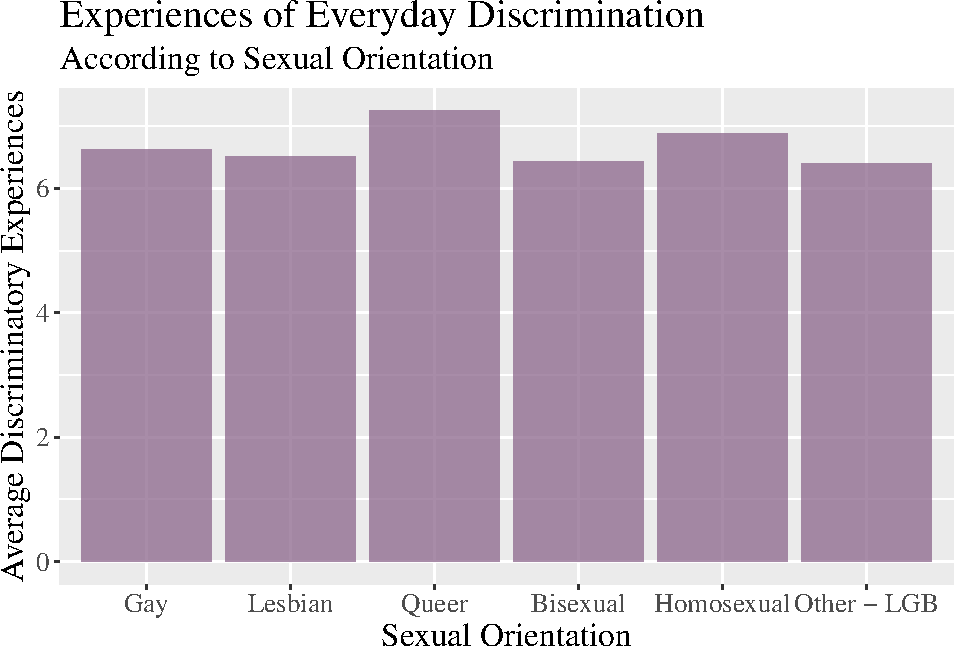
\includegraphics{prep_script_files/figure-latex/mean plot-1.pdf}

\begin{longtable}[]{@{}ll@{}}
\toprule
& stridy (N = 360)\tabularnewline
\midrule
\endhead
\textbf{Everyday Discrmination} & ~~\tabularnewline
~~ min & 0\tabularnewline
~~ median & 7\tabularnewline
~~ max & 8\tabularnewline
~~ mean (sd) & 6.59 ± 1.86\tabularnewline
\textbf{Chronic Strain} & ~~\tabularnewline
~~ min & 1\tabularnewline
~~ median & 1.67\tabularnewline
~~ max & 3\tabularnewline
~~ mean (sd) & 1.71 ± 0.55\tabularnewline
\textbf{Psychological Wellbeing} & ~~\tabularnewline
~~ min & 3\tabularnewline
~~ median & 5.56\tabularnewline
~~ max & 7\tabularnewline
~~ mean (sd) & 5.47 ± 0.79\tabularnewline
\textbf{Social Connectedness} & ~~\tabularnewline
~~ min & 1.38\tabularnewline
~~ median & 3.38\tabularnewline
~~ max & 4\tabularnewline
~~ mean (sd) & 3.29 ± 0.51\tabularnewline
\bottomrule
\end{longtable}

\begin{longtable}[]{@{}lllllll@{}}
\toprule
\begin{minipage}[b]{0.16\columnwidth}\raggedright
\strut
\end{minipage} & \begin{minipage}[b]{0.11\columnwidth}\raggedright
Gay (N = 160)\strut
\end{minipage} & \begin{minipage}[b]{0.11\columnwidth}\raggedright
Lesbian (N = 104)\strut
\end{minipage} & \begin{minipage}[b]{0.11\columnwidth}\raggedright
Queer (N = 12)\strut
\end{minipage} & \begin{minipage}[b]{0.11\columnwidth}\raggedright
Bisexual (N = 63)\strut
\end{minipage} & \begin{minipage}[b]{0.11\columnwidth}\raggedright
Homosexual (N = 16)\strut
\end{minipage} & \begin{minipage}[b]{0.11\columnwidth}\raggedright
Other - LGB (N = 5)\strut
\end{minipage}\tabularnewline
\midrule
\endhead
\begin{minipage}[t]{0.16\columnwidth}\raggedright
\textbf{Everyday Discrmination}\strut
\end{minipage} & \begin{minipage}[t]{0.11\columnwidth}\raggedright
~~\strut
\end{minipage} & \begin{minipage}[t]{0.11\columnwidth}\raggedright
~~\strut
\end{minipage} & \begin{minipage}[t]{0.11\columnwidth}\raggedright
~~\strut
\end{minipage} & \begin{minipage}[t]{0.11\columnwidth}\raggedright
~~\strut
\end{minipage} & \begin{minipage}[t]{0.11\columnwidth}\raggedright
~~\strut
\end{minipage} & \begin{minipage}[t]{0.11\columnwidth}\raggedright
~~\strut
\end{minipage}\tabularnewline
\begin{minipage}[t]{0.16\columnwidth}\raggedright
~~ min\strut
\end{minipage} & \begin{minipage}[t]{0.11\columnwidth}\raggedright
0\strut
\end{minipage} & \begin{minipage}[t]{0.11\columnwidth}\raggedright
0\strut
\end{minipage} & \begin{minipage}[t]{0.11\columnwidth}\raggedright
5\strut
\end{minipage} & \begin{minipage}[t]{0.11\columnwidth}\raggedright
0\strut
\end{minipage} & \begin{minipage}[t]{0.11\columnwidth}\raggedright
0\strut
\end{minipage} & \begin{minipage}[t]{0.11\columnwidth}\raggedright
5\strut
\end{minipage}\tabularnewline
\begin{minipage}[t]{0.16\columnwidth}\raggedright
~~ median\strut
\end{minipage} & \begin{minipage}[t]{0.11\columnwidth}\raggedright
7\strut
\end{minipage} & \begin{minipage}[t]{0.11\columnwidth}\raggedright
7\strut
\end{minipage} & \begin{minipage}[t]{0.11\columnwidth}\raggedright
7\strut
\end{minipage} & \begin{minipage}[t]{0.11\columnwidth}\raggedright
7\strut
\end{minipage} & \begin{minipage}[t]{0.11\columnwidth}\raggedright
8\strut
\end{minipage} & \begin{minipage}[t]{0.11\columnwidth}\raggedright
6\strut
\end{minipage}\tabularnewline
\begin{minipage}[t]{0.16\columnwidth}\raggedright
~~ max\strut
\end{minipage} & \begin{minipage}[t]{0.11\columnwidth}\raggedright
8\strut
\end{minipage} & \begin{minipage}[t]{0.11\columnwidth}\raggedright
8\strut
\end{minipage} & \begin{minipage}[t]{0.11\columnwidth}\raggedright
8\strut
\end{minipage} & \begin{minipage}[t]{0.11\columnwidth}\raggedright
8\strut
\end{minipage} & \begin{minipage}[t]{0.11\columnwidth}\raggedright
8\strut
\end{minipage} & \begin{minipage}[t]{0.11\columnwidth}\raggedright
8\strut
\end{minipage}\tabularnewline
\begin{minipage}[t]{0.16\columnwidth}\raggedright
~~ mean (sd)\strut
\end{minipage} & \begin{minipage}[t]{0.11\columnwidth}\raggedright
6.63 ± 1.72\strut
\end{minipage} & \begin{minipage}[t]{0.11\columnwidth}\raggedright
6.52 ± 1.99\strut
\end{minipage} & \begin{minipage}[t]{0.11\columnwidth}\raggedright
7.25 ± 0.87\strut
\end{minipage} & \begin{minipage}[t]{0.11\columnwidth}\raggedright
6.43 ± 2.13\strut
\end{minipage} & \begin{minipage}[t]{0.11\columnwidth}\raggedright
6.88 ± 2.03\strut
\end{minipage} & \begin{minipage}[t]{0.11\columnwidth}\raggedright
6.40 ± 1.14\strut
\end{minipage}\tabularnewline
\begin{minipage}[t]{0.16\columnwidth}\raggedright
\textbf{Chronic Strain}\strut
\end{minipage} & \begin{minipage}[t]{0.11\columnwidth}\raggedright
~~\strut
\end{minipage} & \begin{minipage}[t]{0.11\columnwidth}\raggedright
~~\strut
\end{minipage} & \begin{minipage}[t]{0.11\columnwidth}\raggedright
~~\strut
\end{minipage} & \begin{minipage}[t]{0.11\columnwidth}\raggedright
~~\strut
\end{minipage} & \begin{minipage}[t]{0.11\columnwidth}\raggedright
~~\strut
\end{minipage} & \begin{minipage}[t]{0.11\columnwidth}\raggedright
~~\strut
\end{minipage}\tabularnewline
\begin{minipage}[t]{0.16\columnwidth}\raggedright
~~ min\strut
\end{minipage} & \begin{minipage}[t]{0.11\columnwidth}\raggedright
1\strut
\end{minipage} & \begin{minipage}[t]{0.11\columnwidth}\raggedright
1\strut
\end{minipage} & \begin{minipage}[t]{0.11\columnwidth}\raggedright
1\strut
\end{minipage} & \begin{minipage}[t]{0.11\columnwidth}\raggedright
1\strut
\end{minipage} & \begin{minipage}[t]{0.11\columnwidth}\raggedright
1\strut
\end{minipage} & \begin{minipage}[t]{0.11\columnwidth}\raggedright
1.33\strut
\end{minipage}\tabularnewline
\begin{minipage}[t]{0.16\columnwidth}\raggedright
~~ median\strut
\end{minipage} & \begin{minipage}[t]{0.11\columnwidth}\raggedright
1.67\strut
\end{minipage} & \begin{minipage}[t]{0.11\columnwidth}\raggedright
1.67\strut
\end{minipage} & \begin{minipage}[t]{0.11\columnwidth}\raggedright
1.5\strut
\end{minipage} & \begin{minipage}[t]{0.11\columnwidth}\raggedright
2\strut
\end{minipage} & \begin{minipage}[t]{0.11\columnwidth}\raggedright
1.33\strut
\end{minipage} & \begin{minipage}[t]{0.11\columnwidth}\raggedright
2\strut
\end{minipage}\tabularnewline
\begin{minipage}[t]{0.16\columnwidth}\raggedright
~~ max\strut
\end{minipage} & \begin{minipage}[t]{0.11\columnwidth}\raggedright
3\strut
\end{minipage} & \begin{minipage}[t]{0.11\columnwidth}\raggedright
3\strut
\end{minipage} & \begin{minipage}[t]{0.11\columnwidth}\raggedright
3\strut
\end{minipage} & \begin{minipage}[t]{0.11\columnwidth}\raggedright
2.67\strut
\end{minipage} & \begin{minipage}[t]{0.11\columnwidth}\raggedright
1.67\strut
\end{minipage} & \begin{minipage}[t]{0.11\columnwidth}\raggedright
2.67\strut
\end{minipage}\tabularnewline
\begin{minipage}[t]{0.16\columnwidth}\raggedright
~~ mean (sd)\strut
\end{minipage} & \begin{minipage}[t]{0.11\columnwidth}\raggedright
1.65 ± 0.53\strut
\end{minipage} & \begin{minipage}[t]{0.11\columnwidth}\raggedright
1.77 ± 0.58\strut
\end{minipage} & \begin{minipage}[t]{0.11\columnwidth}\raggedright
1.64 ± 0.61\strut
\end{minipage} & \begin{minipage}[t]{0.11\columnwidth}\raggedright
1.88 ± 0.51\strut
\end{minipage} & \begin{minipage}[t]{0.11\columnwidth}\raggedright
1.35 ± 0.26\strut
\end{minipage} & \begin{minipage}[t]{0.11\columnwidth}\raggedright
1.87 ± 0.56\strut
\end{minipage}\tabularnewline
\begin{minipage}[t]{0.16\columnwidth}\raggedright
\textbf{Psychological Wellbeing}\strut
\end{minipage} & \begin{minipage}[t]{0.11\columnwidth}\raggedright
~~\strut
\end{minipage} & \begin{minipage}[t]{0.11\columnwidth}\raggedright
~~\strut
\end{minipage} & \begin{minipage}[t]{0.11\columnwidth}\raggedright
~~\strut
\end{minipage} & \begin{minipage}[t]{0.11\columnwidth}\raggedright
~~\strut
\end{minipage} & \begin{minipage}[t]{0.11\columnwidth}\raggedright
~~\strut
\end{minipage} & \begin{minipage}[t]{0.11\columnwidth}\raggedright
~~\strut
\end{minipage}\tabularnewline
\begin{minipage}[t]{0.16\columnwidth}\raggedright
~~ min\strut
\end{minipage} & \begin{minipage}[t]{0.11\columnwidth}\raggedright
3\strut
\end{minipage} & \begin{minipage}[t]{0.11\columnwidth}\raggedright
3.41\strut
\end{minipage} & \begin{minipage}[t]{0.11\columnwidth}\raggedright
4.29\strut
\end{minipage} & \begin{minipage}[t]{0.11\columnwidth}\raggedright
3.18\strut
\end{minipage} & \begin{minipage}[t]{0.11\columnwidth}\raggedright
3.12\strut
\end{minipage} & \begin{minipage}[t]{0.11\columnwidth}\raggedright
3.88\strut
\end{minipage}\tabularnewline
\begin{minipage}[t]{0.16\columnwidth}\raggedright
~~ median\strut
\end{minipage} & \begin{minipage}[t]{0.11\columnwidth}\raggedright
5.62\strut
\end{minipage} & \begin{minipage}[t]{0.11\columnwidth}\raggedright
5.53\strut
\end{minipage} & \begin{minipage}[t]{0.11\columnwidth}\raggedright
6.03\strut
\end{minipage} & \begin{minipage}[t]{0.11\columnwidth}\raggedright
5.24\strut
\end{minipage} & \begin{minipage}[t]{0.11\columnwidth}\raggedright
5.74\strut
\end{minipage} & \begin{minipage}[t]{0.11\columnwidth}\raggedright
5.12\strut
\end{minipage}\tabularnewline
\begin{minipage}[t]{0.16\columnwidth}\raggedright
~~ max\strut
\end{minipage} & \begin{minipage}[t]{0.11\columnwidth}\raggedright
7\strut
\end{minipage} & \begin{minipage}[t]{0.11\columnwidth}\raggedright
6.82\strut
\end{minipage} & \begin{minipage}[t]{0.11\columnwidth}\raggedright
7\strut
\end{minipage} & \begin{minipage}[t]{0.11\columnwidth}\raggedright
6.82\strut
\end{minipage} & \begin{minipage}[t]{0.11\columnwidth}\raggedright
6.59\strut
\end{minipage} & \begin{minipage}[t]{0.11\columnwidth}\raggedright
5.76\strut
\end{minipage}\tabularnewline
\begin{minipage}[t]{0.16\columnwidth}\raggedright
~~ mean (sd)\strut
\end{minipage} & \begin{minipage}[t]{0.11\columnwidth}\raggedright
5.51 ± 0.79\strut
\end{minipage} & \begin{minipage}[t]{0.11\columnwidth}\raggedright
5.53 ± 0.70\strut
\end{minipage} & \begin{minipage}[t]{0.11\columnwidth}\raggedright
5.75 ± 0.78\strut
\end{minipage} & \begin{minipage}[t]{0.11\columnwidth}\raggedright
5.24 ± 0.85\strut
\end{minipage} & \begin{minipage}[t]{0.11\columnwidth}\raggedright
5.47 ± 1.01\strut
\end{minipage} & \begin{minipage}[t]{0.11\columnwidth}\raggedright
4.95 ± 0.72\strut
\end{minipage}\tabularnewline
\begin{minipage}[t]{0.16\columnwidth}\raggedright
\textbf{Social Connectedness}\strut
\end{minipage} & \begin{minipage}[t]{0.11\columnwidth}\raggedright
~~\strut
\end{minipage} & \begin{minipage}[t]{0.11\columnwidth}\raggedright
~~\strut
\end{minipage} & \begin{minipage}[t]{0.11\columnwidth}\raggedright
~~\strut
\end{minipage} & \begin{minipage}[t]{0.11\columnwidth}\raggedright
~~\strut
\end{minipage} & \begin{minipage}[t]{0.11\columnwidth}\raggedright
~~\strut
\end{minipage} & \begin{minipage}[t]{0.11\columnwidth}\raggedright
~~\strut
\end{minipage}\tabularnewline
\begin{minipage}[t]{0.16\columnwidth}\raggedright
~~ min\strut
\end{minipage} & \begin{minipage}[t]{0.11\columnwidth}\raggedright
1.38\strut
\end{minipage} & \begin{minipage}[t]{0.11\columnwidth}\raggedright
2.12\strut
\end{minipage} & \begin{minipage}[t]{0.11\columnwidth}\raggedright
3.25\strut
\end{minipage} & \begin{minipage}[t]{0.11\columnwidth}\raggedright
1.88\strut
\end{minipage} & \begin{minipage}[t]{0.11\columnwidth}\raggedright
2.62\strut
\end{minipage} & \begin{minipage}[t]{0.11\columnwidth}\raggedright
2.12\strut
\end{minipage}\tabularnewline
\begin{minipage}[t]{0.16\columnwidth}\raggedright
~~ median\strut
\end{minipage} & \begin{minipage}[t]{0.11\columnwidth}\raggedright
3.25\strut
\end{minipage} & \begin{minipage}[t]{0.11\columnwidth}\raggedright
3.38\strut
\end{minipage} & \begin{minipage}[t]{0.11\columnwidth}\raggedright
3.44\strut
\end{minipage} & \begin{minipage}[t]{0.11\columnwidth}\raggedright
3.12\strut
\end{minipage} & \begin{minipage}[t]{0.11\columnwidth}\raggedright
3.5\strut
\end{minipage} & \begin{minipage}[t]{0.11\columnwidth}\raggedright
2.75\strut
\end{minipage}\tabularnewline
\begin{minipage}[t]{0.16\columnwidth}\raggedright
~~ max\strut
\end{minipage} & \begin{minipage}[t]{0.11\columnwidth}\raggedright
4\strut
\end{minipage} & \begin{minipage}[t]{0.11\columnwidth}\raggedright
4\strut
\end{minipage} & \begin{minipage}[t]{0.11\columnwidth}\raggedright
4\strut
\end{minipage} & \begin{minipage}[t]{0.11\columnwidth}\raggedright
4\strut
\end{minipage} & \begin{minipage}[t]{0.11\columnwidth}\raggedright
3.88\strut
\end{minipage} & \begin{minipage}[t]{0.11\columnwidth}\raggedright
3.75\strut
\end{minipage}\tabularnewline
\begin{minipage}[t]{0.16\columnwidth}\raggedright
~~ mean (sd)\strut
\end{minipage} & \begin{minipage}[t]{0.11\columnwidth}\raggedright
3.26 ± 0.54\strut
\end{minipage} & \begin{minipage}[t]{0.11\columnwidth}\raggedright
3.41 ± 0.45\strut
\end{minipage} & \begin{minipage}[t]{0.11\columnwidth}\raggedright
3.51 ± 0.25\strut
\end{minipage} & \begin{minipage}[t]{0.11\columnwidth}\raggedright
3.14 ± 0.51\strut
\end{minipage} & \begin{minipage}[t]{0.11\columnwidth}\raggedright
3.38 ± 0.40\strut
\end{minipage} & \begin{minipage}[t]{0.11\columnwidth}\raggedright
2.95 ± 0.71\strut
\end{minipage}\tabularnewline
\bottomrule
\end{longtable}

\hypertarget{primary-analyses}{%
\subsection{Primary Analyses}\label{primary-analyses}}

A multiple regression analysis was conducted to examine the effects of discriminatory experiences, chronic strain, social connectedness on psychological wellbeing among LGBQ individuals. When all variables were entered into the model, discriminatory experiences was negatively associated with psychological wellbeing, \(\hat{\beta_{1}}=-0.05, SE(\hat{\beta_{1}})=-0.11, t(356)=-2.14, p=.03\). Likewise, consistent with hypothesis 2, chronic strain was significantly negatively associated with psychological wellbeing,\(\hat{\beta_{2}}=-0.29, SE(\hat{\beta_{2}})=-0.20, t(356)=-3.91, p < .001\). Consistent with hypothesis 3, social connectedness was significantly positively associated with psychological wellbeing,\(\hat{\beta_{3}}=0.24, SE(\hat{\beta_{3}})=0.15, t(356)=2.99, p < .001\). Taken together, all three predictors explained approximately 7.7\% of the variance in psychological wellbeing,\(F(3,356)=9.90, p<.001, R^{2}=.077\).

Call:
lm(formula = perwellb\_2 \textasciitilde{} 1 + dis\_d\_total + chr\_gen\_2 + connect,
data = stridy)

Residuals:
Min 1Q Median 3Q Max
-2.35394 -0.45205 0.06373 0.59705 1.47574

Coefficients:
Estimate Standardized Std. Error t value Pr(\textgreater\textbar t\textbar)\\
(Intercept) 5.48365 0.00000 0.32914 16.661 \textless{} 2e-16 \textbf{\emph{
dis\_d\_total -0.04643 -0.10911 0.02167 -2.142 0.032837 }\\
chr\_gen\_2 -0.28802 -0.19891 0.07375 -3.905 0.000113 }*
connect 0.23789 0.15251 0.07945 2.994 0.002944 **
---
Signif. codes: 0 `\emph{\textbf{' 0.001 '}' 0.01 '}' 0.05 `.' 0.1 ' ' 1

Residual standard error: 0.7633 on 356 degrees of freedom
Multiple R-squared: 0.077, Adjusted R-squared: 0.06922
F-statistic: 9.9 on 3 and 356 DF, p-value: 2.764e-06

ANOVA results using perwellb\_2 as the dependent variable

Predictor SS df MS F p partial\_eta2 CI\_90\_partial\_eta2
(Intercept) 161.70 1 161.70 277.58 .000\\
dis\_d\_total 2.67 1 2.67 4.59 .033 .01 {[}.00, .04{]}
chr\_gen\_2 8.89 1 8.89 15.25 .000 .04 {[}.01, .08{]}
connect 5.22 1 5.22 8.97 .003 .02 {[}.00, .06{]}
Error 207.39 356 0.58

Note: Values in square brackets indicate the bounds of the 90\% confidence interval for partial eta-squared

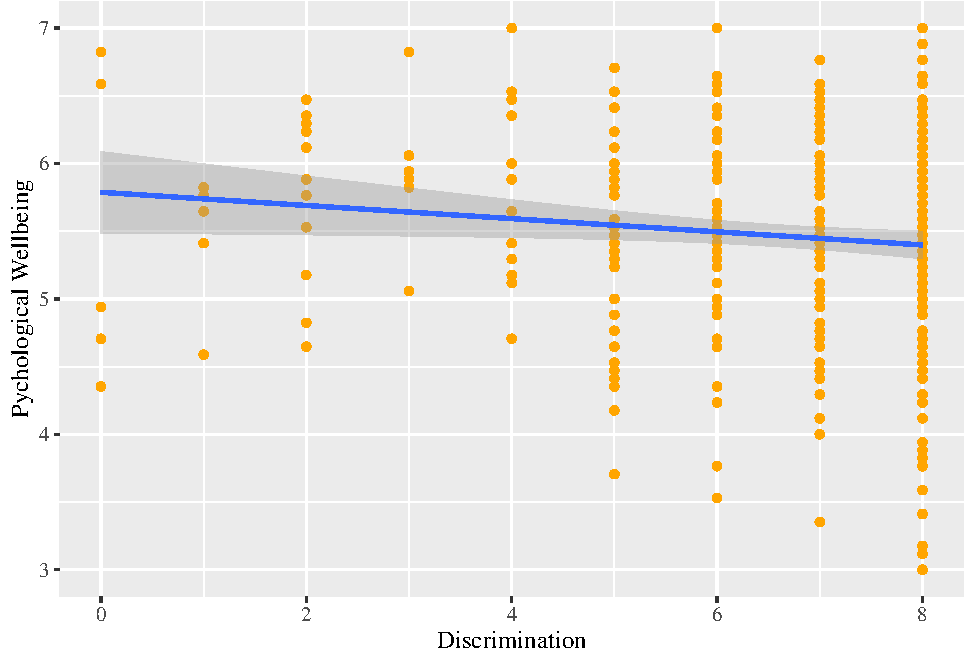
\includegraphics{prep_script_files/figure-latex/regression-1.pdf}

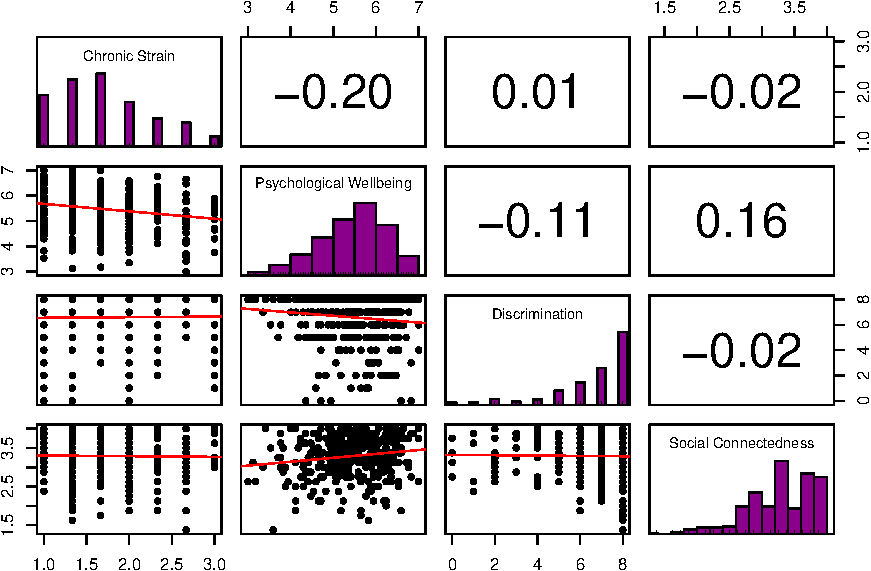
\includegraphics{prep_script_files/figure-latex/correlation panels-1.pdf} chr\_gen\_2 perwellb\_2 dis\_d\_total connect
chr\_gen\_2 1.000 -0.203 0.014 -0.019
perwellb\_2 -0.203 1.000 -0.114 0.158
dis\_d\_total 0.014 -0.114 1.000 -0.016
connect -0.019 0.158 -0.016 1.000

\begin{verbatim}
## lavaan 0.6-7 ended normally after 14 iterations
## 
##   Estimator                                         ML
##   Optimization method                           NLMINB
##   Number of free parameters                          4
##                                                       
##   Number of observations                           360
##                                                       
## Model Test User Model:
##                                                       
##   Test statistic                                 0.000
##   Degrees of freedom                                 0
## 
## Parameter Estimates:
## 
##   Standard errors                             Standard
##   Information                                 Expected
##   Information saturated (h1) model          Structured
## 
## Regressions:
##                    Estimate  Std.Err  z-value  P(>|z|)
##   perwellb_2 ~                                        
##     dis_d_total      -0.046    0.022   -2.154    0.031
##     chr_gen_2        -0.288    0.073   -3.927    0.000
##     connect           0.238    0.079    3.011    0.003
## 
## Variances:
##                    Estimate  Std.Err  z-value  P(>|z|)
##    .perwellb_2        0.576    0.043   13.416    0.000
\end{verbatim}

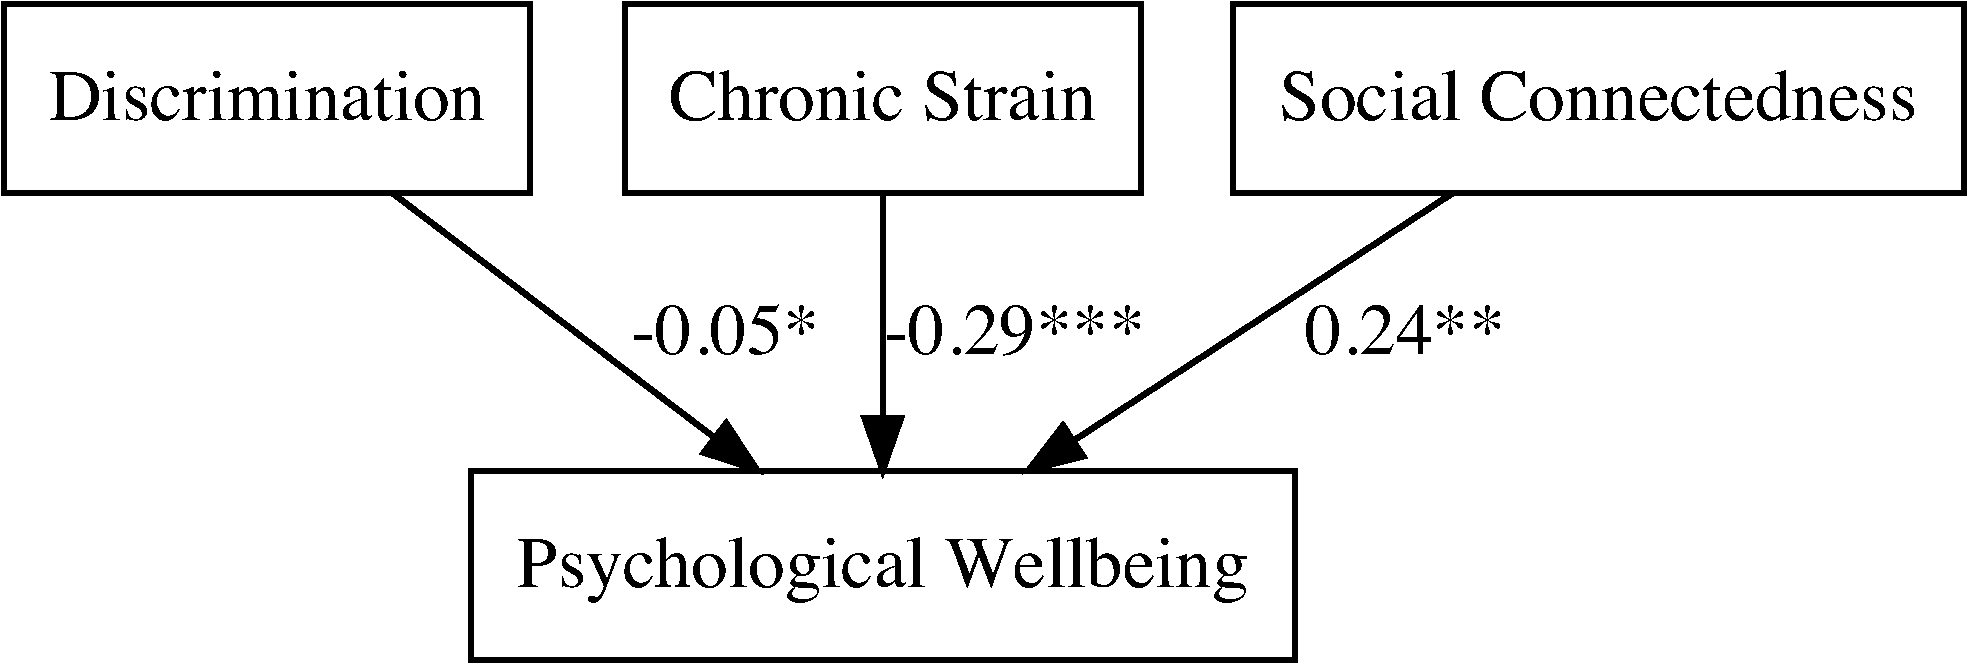
\includegraphics{prep_script_files/figure-latex/lavaan plot-1.pdf}

\hypertarget{discussion}{%
\section{Discussion}\label{discussion}}

\newpage

\hypertarget{references}{%
\section{References}\label{references}}

\begingroup
\setlength{\parindent}{-0.5in}
\setlength{\leftskip}{0.5in}

\hypertarget{refs}{}
\begin{CSLReferences}{0}{0}
\end{CSLReferences}

\endgroup


\printbibliography

\end{document}
